На рисунках 
\ref{fig:BPS_Catia_Top}--\ref{fig:BPS_Catia_Front} показана модель гипотетической конструкции БПЛА.


\begin{figure}[H]
\centering
\def\svgwidth{0.9\textwidth}
\input{figures/BPS_Catia_Top.pdf_tex}
\caption{Вид сверху}
\label{fig:BPS_Catia_Top}
\end{figure}

Как видно из рисунков, для данной компоновочной схемы используется крыло большого удлинения. Из рисунка \ref{fig:BPS_Catia_WithoutSkin}, на котором представлена базовая конструктивно-силовая схема БПЛА, можно видеть, как происходит интеграция корпуса фюзеляжа, крыла и двигателя. 

\begin{figure}[H]
\centering
\input{figures/BPS_Catia_Front.pdf_tex}
%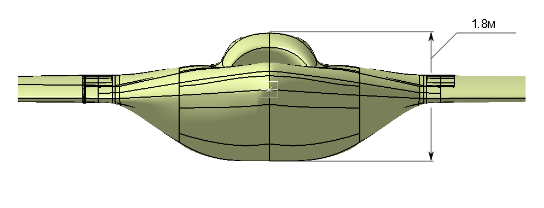
\includegraphics[width=0.8\textwidth]{BPS_Catia_Front}
\caption{Вид фюзеляжа спереди}
\label{fig:BPS_Catia_Front}
\end{figure}

\begin{figure}[H]
\centering
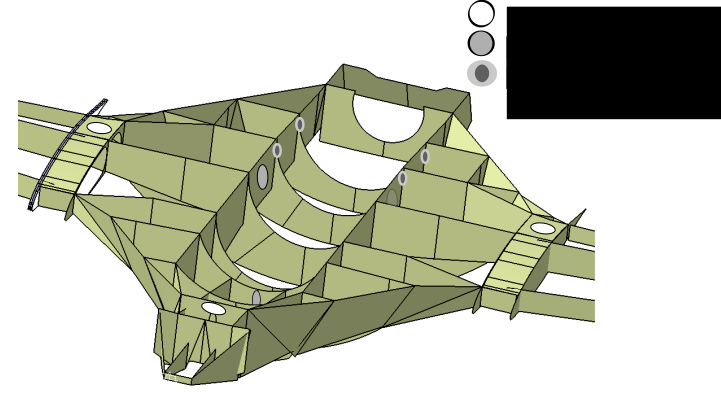
\includegraphics[width=0.8\textwidth]{BPS_Catia_WithoutSkin}
\caption{Вид фюзеляжа со снятой обшивкой}
\label{fig:BPS_Catia_WithoutSkin}
\end{figure}

%\begin{figure}[H]
%\centering
%\def\svgwidth{0.9\textwidth}
%\input{figures/BPS_Catia_WithoutSkin.pdf_tex}
%\caption{Вид фюзеляжа со снятой обшивкой с указанием узлов крепления шасси и двигателя}
%\label{fig:BPS_Catia_WithoutSkin}
%\end{figure}

Из рисунков видно, что двигатель с воздухозаборником значительно утоплены и находятся практически в середине фюзеляжа. Как уже отмечалось выше, эта особенность позволяет значительно улучшить малозаметность и аэродинамическое качество самолета (ссылка на отчет), но приводит к необходимости формировать искривленный центроплан. 

Формирование искривленного центроплана создает дополнительные проблемы прочности из-за большой величины изгибающего момента в корне крыла. Еще одной проблемой обеспечения прочности корпуса БПЛА является высокая чувствительность параметров управляемости БПЛА к изменению жесткостных характеристик корпуса и особенно зоны стыка крыла с центропланом, где расположены узлы крепления стоек основного шасси. Очевидно, что для решения проектировочной задачи необходимо проведение комплексных исследований прочности данной конструкции включая анализ прочности, устойчивости и управляемости. 

В модели гипотетической конструкции БПЛА отсутствует вертикальное оперение. Горизонтальное оперение представлено рулем высоты. Механизация крыла состоит из расщепляющихся элеронов на концах крыльев, элевонов на средней части крыла и интерцепторов, расположенных ближе к фюзеляжу. В качестве силовой установки используется один реактивный двигатель, углубленный в конструкцию вместе с воздухозаборником. Места креплений стоек и замков шасси, расположение двигателя и узлов его крепления показаны на Рис. \ref{fig:BPS_Catia_Top_WithoutSkin}. 


\begin{figure}[H]
\centering
\def\svgwidth{0.9\textwidth}
\input{figures/BPS_Catia_Top_WithoutSkin.pdf_tex}
\caption{Вид сверху без обшивки с указанием узлов крепления шасси и двигателя}
\label{fig:BPS_Catia_Top_WithoutSkin}
\end{figure}

Отсеки фюзеляжа делятся на несколько групп по назначению. Распределение отсеков фюзеляжа по назначению представлено на Рис.\ref{fig:BPS_Catia_Top_PartRoles}. 

На Рис.\ref{fig:BPS_Catia_Top_PartRoles} схематически показаны основные отсеки конструкции БПЛА. 

\begin{figure}[H]
\centering
\def\svgwidth{0.9\textwidth}
\input{figures/BPS_Catia_Top_PartRoles.pdf_tex}
\caption{Вид сверху с обозначением роли отсеков}
\label{fig:BPS_Catia_Top_PartRoles}
\end{figure}
